%%%%%%%%%%%%%%%%%%%%%%%%%%%%%%%%%%%%%%%%%%%%%%%%%%%%%%%%%%%%%%%%%%%%%%%%%%%%%%%%
%2345678901234567890123456789012345678901234567890123456789012345678901234567890
%        1         2         3         4         5         6         7         8

%\documentclass[letterpaper, 10 pt, conference]{orbieeeconfpre}  % Comment this line out if you need a4paper

\documentclass[a4paper, 10pt, journal]{wissarbIEEE}      % Use this line for a4 paper
%\conference{IEEE Conference for Awesome ORB Research}

\bibliographystyle{orbref-num}

\overrideIEEEmargins                                      % Needed to meet printer requirements.

% See the \addtolength command later in the file to balance the column lengths
% on the last page of the document

\usepackage{hyperref}
\usepackage{graphicx}
\usepackage{tabularx}
\usepackage{booktabs}
\usepackage{lipsum}

\title{\LARGE \bf Feasibility Study - SmartWarehouse}

\author{Felix Hausberger}

\begin{document}
	
	% tense
	% schauen ob die Arbeit einen starken eindruck macht
	% mit der Vorlesung mergen

\maketitle

%%%%%%%%%%%%%%%%%%%%%%%%%%%%%%%%%%%%%%%%%%%%%%%%%%%%%%%%%%%%%%%%%%%%%%%%%%%%%%%%
\begin{abstract}

The background scenario of \textit{SmartWarehouse} offers live video data of a drone with goods in a warehouse, which are to be classified and localized in real time. In the future, this should make it possible to carry out inventories and inventory analyses of a warehouse in a time- and cost-efficient manner conserving resources.

\end{abstract}

%%%%%%%%%%%%%%%%%%%%%%%%%%%%%%%%%%%%%%%%%%%%%%%%%%%%%%%%%%%%%%%%%%%%%%%%%%%%%%%%
\section{Introduction}

Combined with an autonomous drone, modern object detectors could make it possible to conduct inventory checks in the field of warehousing and logistics without human assistance. How different object detectors behave when applied to a real time industry scenario like \textit{SmartWarehouse} should be evaluated in this short paper. As being a feasibility study, the main goal of this work also is to discuss the technical feasibility of the \textit{SmartWarehouse} idea. In \autoref{relatedwork} related work to the two main object detectors should be introduced before explaining the approach and architecture of the \textit{SmartWarehouse} prototype in \autoref{architecture}. In \autoref{evaluation} the results of the feasibility study will be presented and evaluated before the interpretability of the results is discussed in \autoref{discussion}. \autoref{conclusion} gives a quick conclusion about the main achievements of this short paper.

\section{Related Work} \label{relatedwork}

The paper \cite{WeiLiuDragomirAnguelovDumitruErhanChristianSzegedyScottReedChengYangFuAlexander.2016} introduces the \textit{Single Shot MultiBox Detector} (SSD), an object detector reaching up to 76.9\% mean average precision (mAP) while still keeping real time detection characteristics compared to its preceeding competitors like regional convolutional neural networks (R-CNNs). It uses a single neural network to detect objects and creates a set of default bounding boxes over different aspect ratios and scales for each feature map location instead of using an additional bounding box proposal step. 

The \textit{You only Look Once} (YOLO) algorithm was introduced in \cite{JosephRedmonSantoshDivvalaRossGirshickAliFarhadi.2016} and as well uses a single neural network to predict bounding boxes and class probabilities. Incremental improvements led to version three of YOLO, which is equally accurate as SSD, but three times faster \cite{JosephRedmon.2018}. 

\section{Architecture of the SmartWarehouse scenario} \label{architecture}

Two goals were defined for the feasibility study of \textit{SmartWarehouse}. First it is to be evaluated, how well existing object detectors perform in industry scenarios taking the example of \textit{SmartWarehouse} scenario. Second, one should deal with the feasibility of the implementation of this \textit{SmartWarehouse} scenario, which comprises the execution of an inventory for department stores with a drone. 

In the construction of the training dataset, the feasibility study does not aim to completely represent a large department store in the dataset. To prove the general feasibility of the \textit{SmartWarehouse} scenario, it is extensive enough to restrict the focus on unpacked beverage bottles of a department store which can be assigned to nine different classes. All classes are distributed equally among the 1088 manually annotated images. 75\% of the images include a single instances of a beverage bottle to better train the patterns of the different classes. Furthermore, 13\% of the images contain occlusions of objects to be detected, detection situations from extreme viewing positions are represented to 4\%, and difficult illumination and lighting conditions are included to 8\%. Only a few examples (2\%) are related to different distances during detection. Care was also taken to continuously vary the backgrounds of the objects being detected. Finally, to simulate the department store where several objects are to be detected at once, in 12.5\% of all images the objects are arranged on shelves, one behind the other or in beverage crates. 

To better compare object detectors with each other the following evaluation criteria have been defined:

\begin{itemize}
	\item Precision: The precision of an object detector measured in mAP
	\item Reactivity: The inference rate with the model measured in \textit{Frames Per Second} (FPS)
	\item Inference behavior: The inference behavior under special lighting conditions, extreme viewing positions, occultation of objects, and the behavior with double detected objects measured by the confidence score. 
\end{itemize}

For the \textit{SmartWarehouse} scenario, a choice should be made between the four detectors Faster R-CNN, Mask R-CNN, SSD and YOLO. 

\begin{figure}[h]
	\centering
	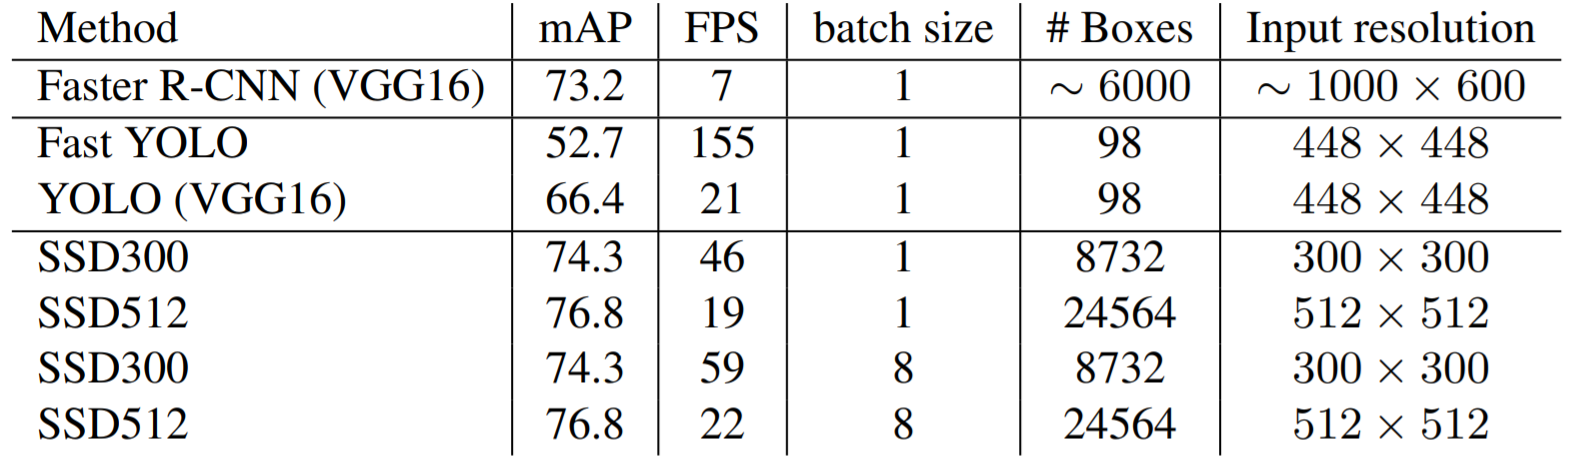
\includegraphics[width=0.5\textwidth]{fig/ssd_results.png}
	\caption{Comparison of SSD on PascalVOC 2007 \cite{WeiLiuDragomirAnguelovDumitruErhanChristianSzegedyScottReedChengYangFuAlexander.2016}}
	\label{ssd_results}
\end{figure}

According to the reference results in \autoref{ssd_results}, it is clear that the SSD performs best in terms of mAP with 74.3\% and 76.8\%, respectively. Faster-RCNN can keep up with 73.2\% in terms of mAP, but with only 7 FPS it is not designed for fast inference. YOLO scores worse than the SSD in both categories, it essentially achieves an mAP of 66.4\% and a frame rate of 21 FPS. The SSD thus manages to maintain a good balance between precision and responsiveness. Comparing Mask-RCNN from the original paper in \cite{KaimingHeGeorgiaGkioxariPiotrDollarRossGirshick.2018} with Faster-RCNN (RoI-Align) results in a mAP difference of 38.2\% to 37.3\%. Only 5 FPS could be reached. As the effort to setup and to adapt Faster-RCNN and Mask-RCNN to be trained on a custom dataset was far higher and the performance in time-critical model inference was poorer, YOLO and SSD were selected as the two detectors to evaluate the capability of object detectors for industrial use.

Analyzing the market for programmable drones with a freely available software development kit (SDK) and integrated camera, the supply is very low. The choice restricts to either the \textit{Parot Bebop II} or the \textit{Ryze Tello EDU}. When also taking into account the legal framework, only the \textit{Ryze Tello EDU} was left for legal usage.

To process the drone's image data for an inventory, the drone is to be accessed by a client application. The server, acting as a client, is to connect to the drone and sends the flight signals as static flight instructions to the drone. The deep learning model is also to be integrated on the server for inference. The server's task will be to infer the video stream frames received from the drone with the model, count the detected objects for the inventory using a counting algorithm, and then forward the image data with the bounding boxes drawn in via livestream to a web application for visualization. A REST interface should provide information about the inventory data of the warehouse and provide a way to initiate the flight sequence.

\section{Results and evaluation} \label{evaluation}

SSD reached an mAP score of 83.1\%, while YOLO scores almost equally high with 80.4\%. To minimize double detected objects the confidence score for SSD was set to 0.7, for YOLO already 0.25 was enough. SDD struggles to detect partly hidden objects. Also detecting objects from extreme view positions was difficult, but can be improved by adding more samples for this case. For those special cases YOLO performs equally bad, for the latter even worse. SSD reliably detects objects until a three meters distance threshold, YOLOs' maximum range is only two meters. Overlit lighting conditions leads to no or wrong object detection using the SSD or YOLO algorithm. However, all detections of both models reacted invariantly to different backgrounds or image resolutions. Both SSD and YOLO are capable to run inference in the real time scenario of \textit{SmartWarehouse}, SSD with 30 PFS and YOLO with 28 FPS. 

\section{Discussion} \label{discussion}

In terms of precision, both object detectors turn out better than the original reference results from the scientific publications. However, it should be noted that the results do not compare well with those of the scientific publications, since they were trained on different, significantly simpler data. With 83.1\%, SSD300 is 8.8\% better, while YOLOv3 even shows an improvement of 16.7\%. Nevertheless, it can be concluded that both implementations scale in terms of precision in an order of magnitude that comes after the level of the comparison results from PascalVOC 2007.

Another evaluation criterion is the responsiveness. Here, SSD300 scores slightly better with an average of 30 FPS than YOLOv3 with 28 FPS, although this difference should hardly be seen as a true decision criterion to prefer SSD300 over YOLOv3.

Regarding inference behavior both object detectors struggle with difficult lightning conditions, extreme viewing positions, longer distances and occlusions. Some of those problems could be tackled better by enhancing the dataset with additional instances for those cases.
 
Overall, it can be concluded that both SSD300 and YOLOv3 are object detectors for industrial use. If many objects of different scales are to be detected in the detection environment, SSD300 is preferable to YOLOv3. However, if this is not the case and more emphasis is placed on accuracy for simple datasets such as \textit{SmartWarehouse}, YOLOv3 is the better choice.

When evaluating the technical feasibility of the \textit{SmartWarehouse} scenario, three issues remained unsolved:

\begin{itemize}
	\item Inferring the video stream of the drone, due to the incompatibility of the runtime environments for the H.264 decoder and the deep learning models,
	\item The detection of occluded objects, and
	\item The unique counting of objects during the inventory.
\end{itemize}

The \textit{SmartWarehouse} scenario is therefore not feasible according to the decisions made and with the given framework conditions.

\section{Conclusion} \label{conclusion}

The goal of this work was to evaluate how well existing object detectors are basically suited for industrial application scenarios, and to determine whether the specific application scenario for conducting an inventory of department stores using a drone can be implemented as a prototype. 

Even if object detectors such as SSD and YOLO most certainly have the potential to be used industrially, the \textit{SmartWarehouse} scenario still could not be realized end-to-end. To do so, one would need to enhance the dataset to cover certain image capturing conditions as described, implement a custom H.264 decoder to connect the drone video stream to the selected deep learning model for real time inference and find a solution to uniquely identify objects during the detection process like additionaly making use of RFID technology. 

\bibliography{mybibfile}

\end{document}